\documentclass{beamer}
\usepackage[utf8]{inputenc}
\usepackage{graphicx}
\usepackage{hyperref}
\usepackage{amsmath,amssymb}
% \usepackage{geometry}
\usepackage{tikz}
\usepackage{multicol}
\usetheme{Boadilla}
\graphicspath{{../../thesis/}}

\newcommand{\Hi}{\textsc{Hi}}
\newcommand{\mHi}{\ensuremath{m_{\Hi}}}

\newcommand{\p}{\ensuremath{\partial}}

\newcommand{\Msun}{\ensuremath{M_{\odot}}}
\newcommand{\Mh}{\ensuremath{h^{-1}M_{\odot}}}
\newcommand{\Mhsq}{\ensuremath{h^{-2}M_{\odot}}}
\newcommand{\Mpch}{\ensuremath{h^{-1}{\rm Mpc}}}
\newcommand{\kpch}{\ensuremath{h^{-1}{\rm kpc}}}
\newcommand{\kms}{\ensuremath{{\rm km\,s}^{-1}}}
\newcommand{\msq}{\ensuremath{{\rm \,m\,s}^{-2}}}

\newcommand{\avg}[1]{\ensuremath{\left\langle \,#1\, \right\rangle}}
\newcommand{\e}[1]{\ensuremath{{\rm e}^{#1}}}

\newcommand{\der}{\ensuremath{{\rm d}}}
\newcommand{\Der}{\ensuremath{{\rm D}}}
\newcommand{\dir}{\ensuremath{\delta_{\rm D}}}

\newcommand{\erfc}[1]{\ensuremath{{\rm erfc}\left(#1\right)}}
\newcommand{\erf}[1]{\ensuremath{{\rm erf}\left(#1\right)}}

\title[Research Overview]{Research Overview and Future Directions}
\author[Premvijay Velmani]{Premvijay Velmani \\ \texttt{premv@iucaa.in}}
\institute[IUCAA]{Inter-University Centre for Astronomy and Astrophysics (IUCAA)}
\date[Interview with Prof Raul Angulo]{January 17, 2025}

\begin{document}

% Title Slide
\begin{frame}
    \titlepage
\end{frame}

% \begin{frame}{Introduction}
% \begin{itemize}

% \end{itemize}    
% \end{frame}

% Slide 1: Introduction
\begin{frame}{Introduction}
\begin{itemize}
\item My research at IUCAA, Pune, mainly involves performing and analysing cosmological simulations with and without galactic astrophysics.
\item Along with simulations, I do more controlled numerical experiments with a focus on physical modelling which can then be compared with observations.
\item I have several research plans based on my past research that will directly benefit from the expertise of KIAS and the available simulation data such as HR5. 
\item I am also excited with the kind of research done at KIAS and hence open to collaborate in those projects.
  % \item Current position ends in July 2025.
\end{itemize}
\end{frame}

\begin{frame}{Background}
    \begin{itemize}
        \item Completed Master of Science (MS) from IISER in 2019 with major in Physics and 1 year thesis work in theoretical cosmology.
        \item Joined IUCAA Pune for PhD in August 2019 and did one year gradschool training in modern astrophysics research.
        \item Started working with Prof. Aseem in 2020. I did comprehensive exploration with cosmological simulations for 1 year and proposed my thesis work.
        \item Worked on my thesis "Interplay of galaxy formation and the evolution of dark matter haloes" for 3 years from 2021 to 2024. Now approved for defence in next month.
        \item As I got another year at IUCAA till July 2025, I continued my research after thesis submission and came up with well-defined long-term research plans. 
        \item Recent KIAS Cosmology workshop, got me know more about the interesting research works over there. I am confident that KIAS has sufficient resources and expertise to get interesting results with these research plans.
    \end{itemize}
\end{frame}

% \begin{frame}{Cosmological Simulations}

    
% \end{frame}

\begin{frame}{Exploring large scale structure in cosmological simulations}
\begin{itemize}
    \item I started by performing cosmo simulations with GADGET and GADGET based codes.
    \item Generated transfer function with CAMB and used 2LPT codes to generate initial conditions for cosmo simulations.
    \item Sample figures from initial exploration with cosmological simulations.
\end{itemize}
    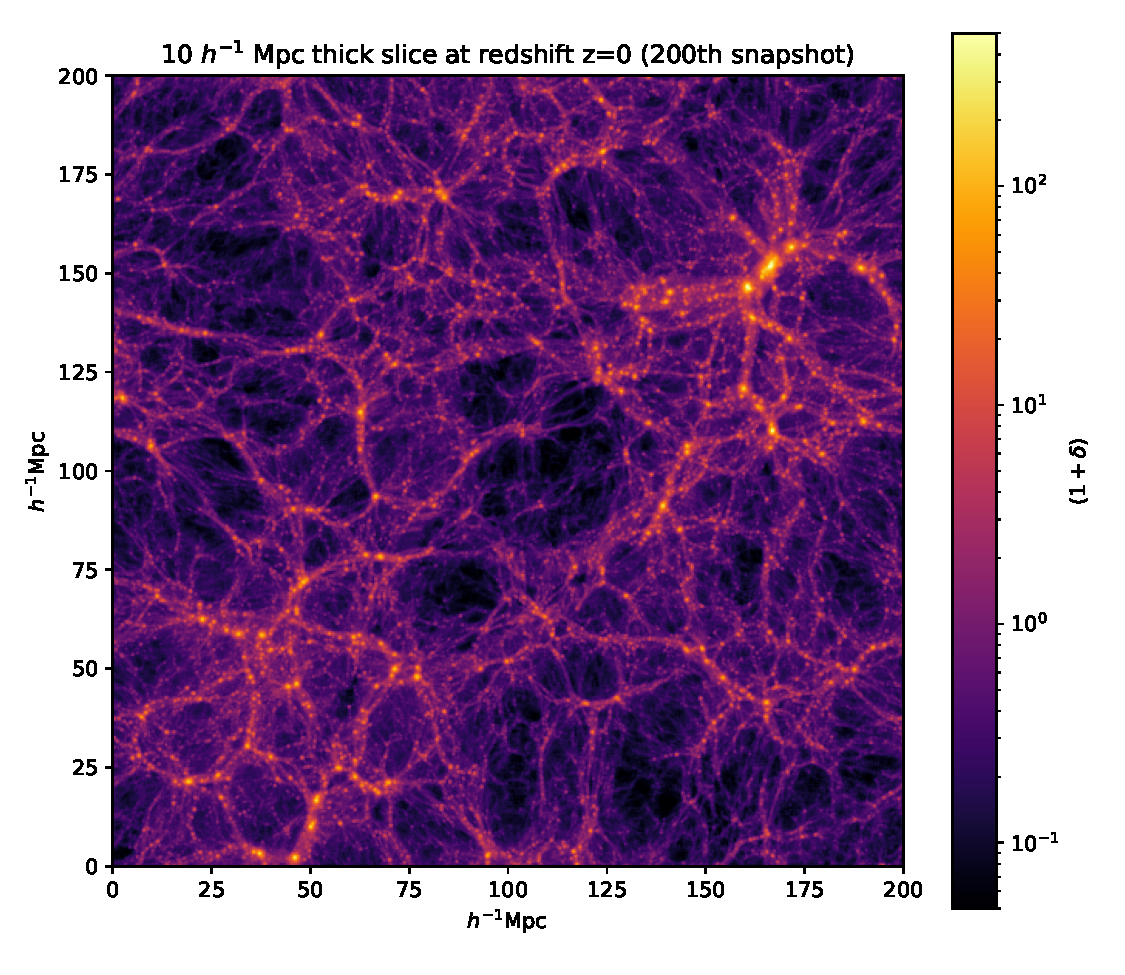
\includegraphics[width=0.485\linewidth]{figures/single_snapshot_image_200_light.pdf}
    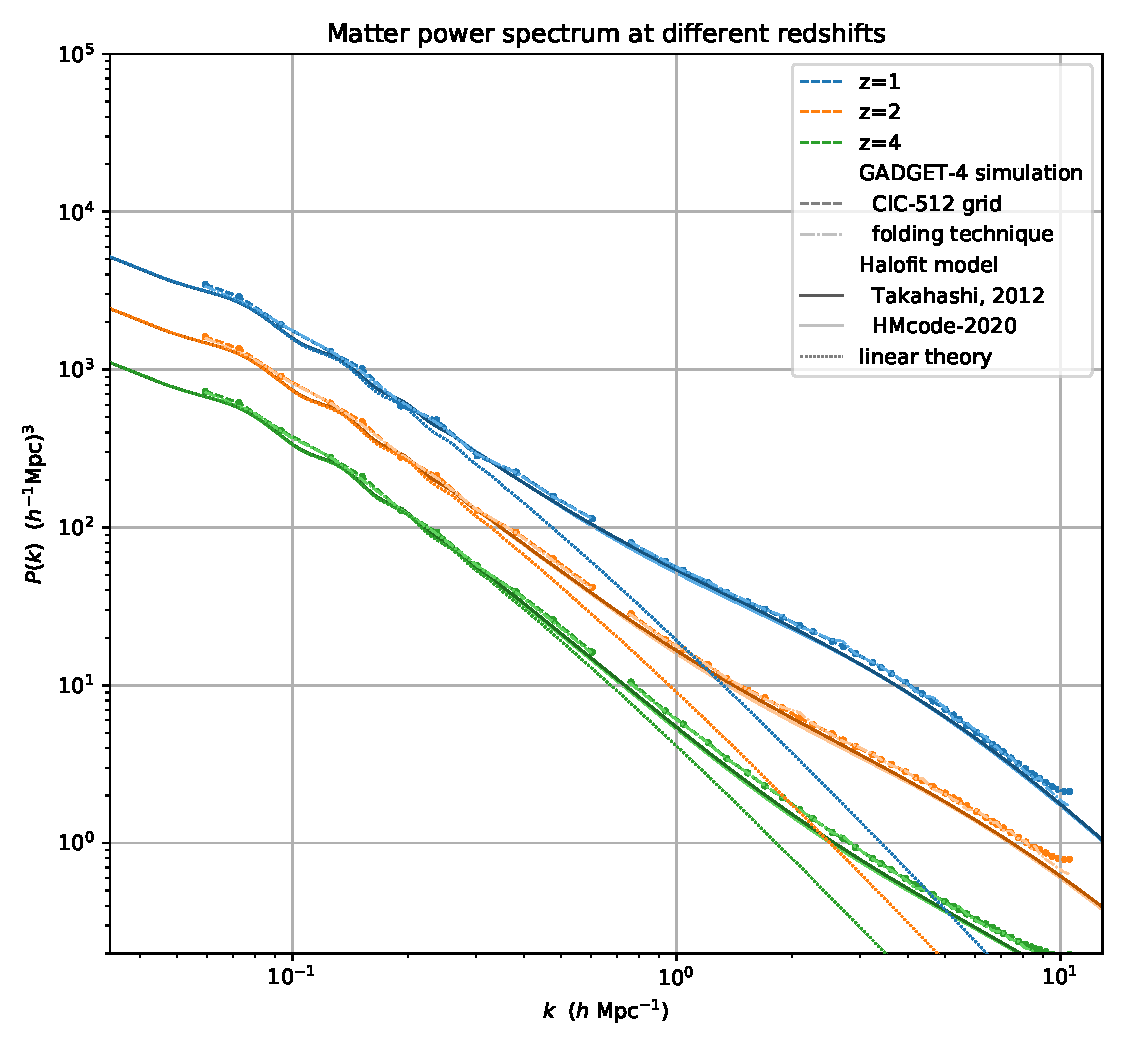
\includegraphics[width=0.485\linewidth]{figures/single_snapshot_pk_vary_z_CIC_light.pdf}
\end{frame}

\begin{frame}{Exploring haloes in galactic and cluster scales}
\begin{itemize}
    \item Found halo substructures with FoF, SUBFIND, ROCKSTAR, VELOCIRAPTOR and built merger trees.
    \item Sample figures from initial exploration with cosmological simulations.
\end{itemize}
    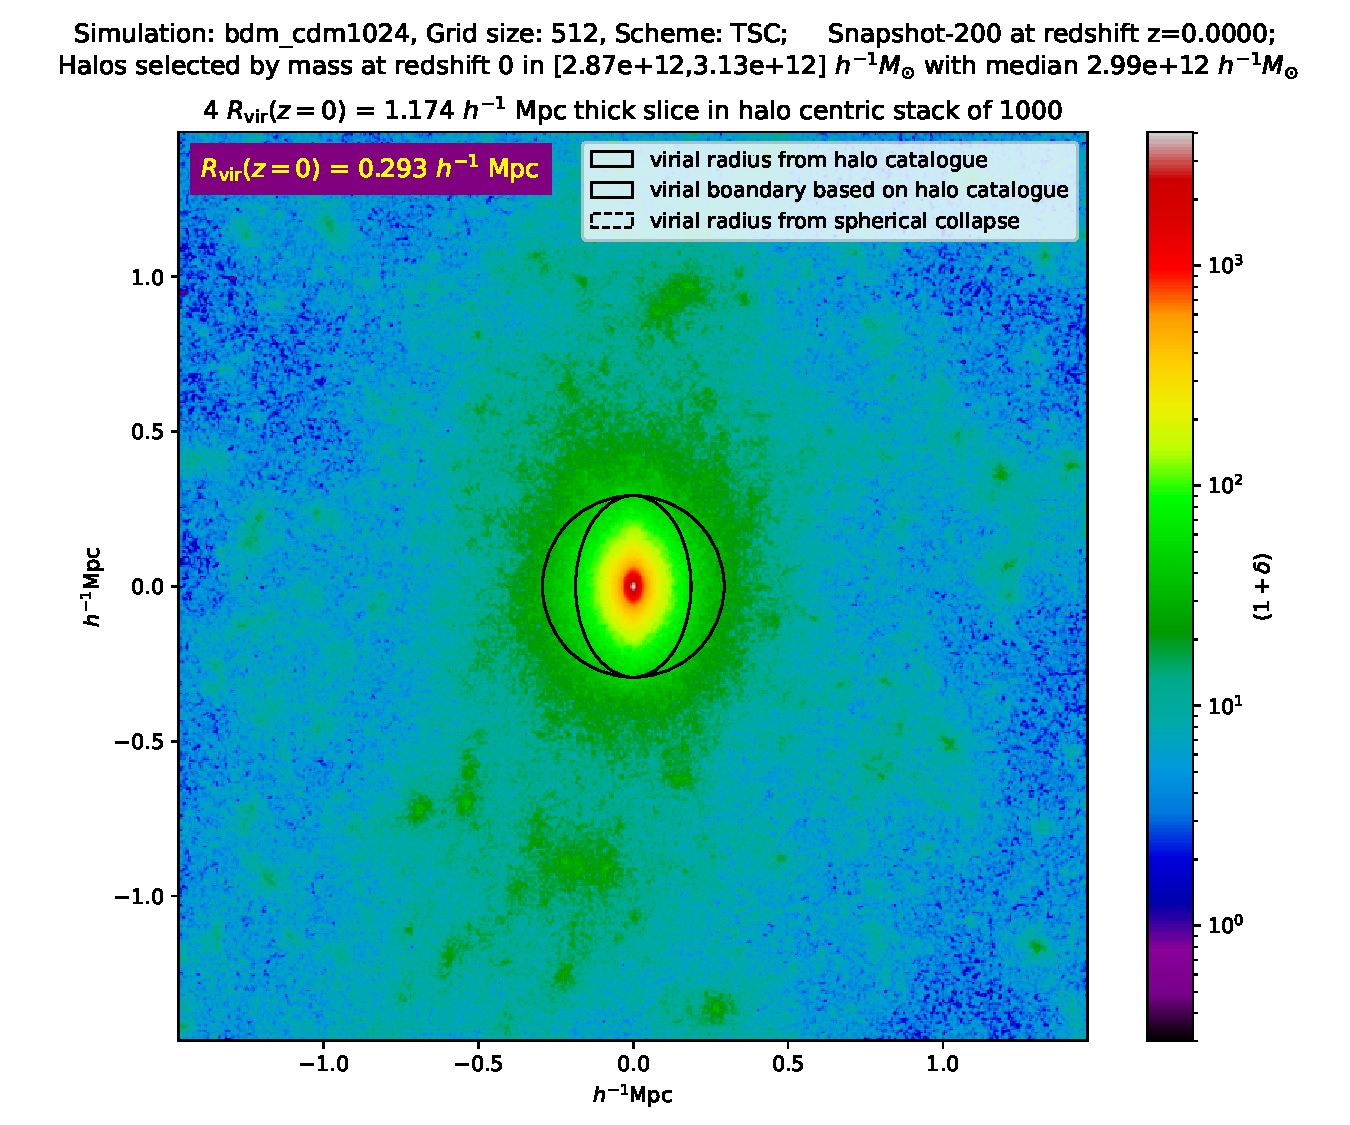
\includegraphics[width=0.485\linewidth]{figures/single_snapshot_200_1by8_3.0e+12_1000_light.pdf}
    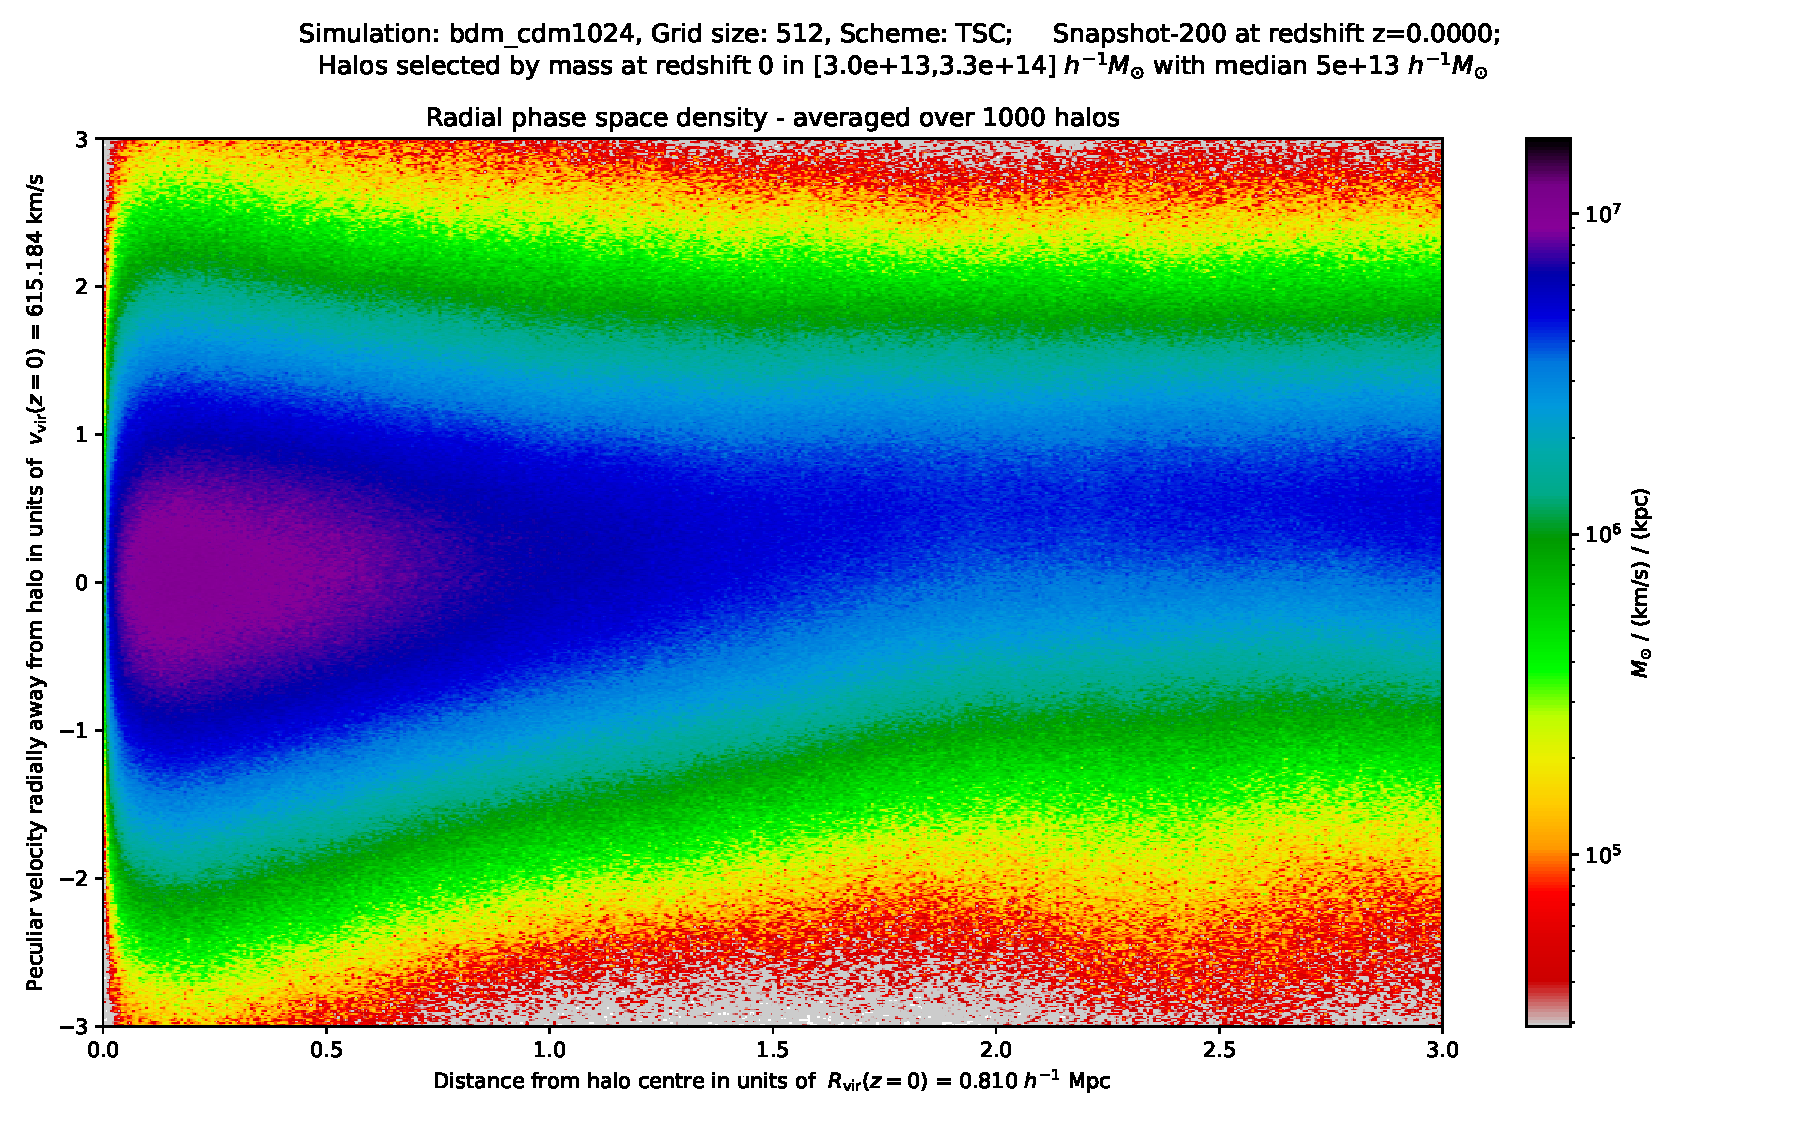
\includegraphics[width=0.485\linewidth]{figures/phase_space_1D_200_1by8_1.0e+14_1000_light.pdf}
\end{frame}



% Slide 2: Past Research - Overview
% \begin{frame}{Past Research: Overview}
%     \begin{itemize}
%         \item Focused on dark matter halo dynamics in cosmological simulations.
%         \item Studied halo relaxation responses using \textbf{IllustrisTNG, EAGLE, and CAMELS}.
%         \item Developed self-similar models for galaxy formation and tested against simulations.
%         \item Analyzed astrophysical feedback processes, especially \textbf{AGN feedback impacts} on halo structure.
%     \end{itemize}
% \end{frame}



\begin{frame}{Hydrodynamical simulations with galaxies} 
\begin{itemize}
    \item In simulations, the phase-space distribution of dark matter within the haloes have also been found to be significantly different and diverse indicating strong response to galaxies they host.
\end{itemize}
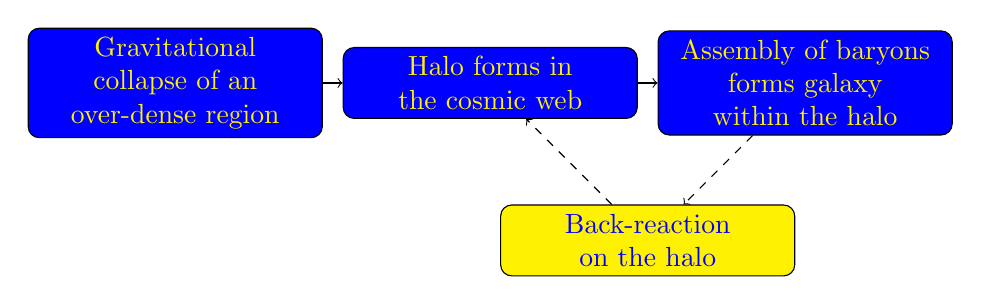
\begin{tikzpicture}[node distance=2cm]
    \node (start) [rectangle, draw, text width=3.5cm, align=center, fill=blue, rounded corners] {\textcolor{yellow}{Gravitational collapse of an over-dense region}};
    \node (halo) [rectangle, draw, right of=start, xshift=2cm, text width=3.5cm, align=center, fill=blue, rounded corners] {\textcolor{yellow}{Halo forms in the cosmic web}};
    \node (galaxy) [rectangle, draw, right of=halo, xshift=2cm, text width=3.5cm, align=center, fill=blue, rounded corners] {\textcolor{yellow}{Assembly of baryons forms galaxy within the halo}};
    
    \draw[->] (start) -- (halo);
    \draw[->] (halo) -- (galaxy);
    
    \node (feedback) [rectangle, draw, below of=halo, xshift=2cm, text width=3.5cm, align=center, fill=yellow, rounded corners] {\textcolor{blue}{Back-reaction on the halo}};
    \draw[->, dashed] (galaxy) -- (feedback);
    \draw[->, dashed] (feedback) -- (halo); 
\end{tikzpicture}
\end{frame}

\begin{frame}{Dark matter halo response to galaxies}
    A halo from EAGLE simulation in the presence of galaxy (left image) can be seen more compact, spherical and even their centres shifted.
    \begin{center}
        \includegraphics[clip,trim={0.5cm 0cm 2cm 0.5cm}, width=0.8\linewidth]{plots/visual_single_halo_E.pdf}
    \end{center} 
    In particular, the change in the halo-centric distances affects radial mass profiles of haloes that influence key observables such as the rotation curves and radial acceleration relations.
\end{frame}


\begin{frame}{Relaxation response in IllustrisTNG and EAGLE}
\begin{columns}
\begin{column}{0.54\linewidth}
    \begin{itemize}
        \item Early works modeled this as adiabatic relaxation of dark matter in response to the net change in the gravitational potential due to galaxy formation.
        \item Quasi-adiabatic relaxation framework focus on modelling the relation between the relaxation ratio $r_f/r_i$ as a function of the mass ratio $M_i/M_f$.
        \item We found that the relaxation relation (between $r_f/r_i$ and $M_i/M_f$) varies widely between haloes of different mass scales in simulations like IllustrisTNG and EAGLE.
    \end{itemize}
    
\end{column}
\begin{column}{0.45\linewidth}
    \begin{center}
        \includegraphics[width=0.99\linewidth]{plots/fit_view_M_T.pdf}
    \end{center}
    \begin{center}
        \includegraphics[width=0.55\linewidth]{plots/Mass_bin_labels_enlarged.pdf}
    \end{center}
\end{column}
\end{columns}
\end{frame}

\begin{frame}{Dependence on halo centric distance}
\begin{itemize}
    \item A simple linear relation can accurately describe the relaxation, provided we assume an additional explicit dependence on the halo-centric distance (indicated by colorbar).
\end{itemize}
\begin{center}
    \includegraphics[clip,trim={0cm 0cm 0.5cm 0.3cm},width=0.32\linewidth]{plots/fit_show_rf_M_T100_M12.5.pdf}
    \includegraphics[width=0.32\linewidth]{plots/fit_show_rf_M_T50_M11.pdf}
    \includegraphics[width=0.32\linewidth]{plots/fit_show_rf_M_E25_M11.pdf}
\end{center}
\end{frame}


\begin{frame}{Universal description of Halo Relaxation Response}
    The radially dependent slope $q_1(r_f)$ and intercept $q_0(r_f)$ of this linear fit, is more universal across a wide range of halo masses up to $10^{13} \Mh$ at $z=0$ (left) and up to $10^{14} \Mh$ at earlier redshift, $z=1$ (right).
    \begin{center}
        \includegraphics[width=0.48\linewidth,trim={0.5cm 0 0 0},clip]{plots/fit_params_rf_M_T_snap098.pdf}
        \includegraphics[width=0.48\linewidth,trim={0.5cm 0 0 0},clip]{plots/fit_params_rf_M_T_snap049_smpl98_allHalsMrange.pdf}
        \hspace{-3.8cm}\raisebox{2.4cm}{\includegraphics[width=0.28\linewidth]{plots/Mass_bin_labels_enlarged.pdf}}\hspace{20cm}
    \end{center}
\end{frame}



\begin{frame}{Relaxation Dynamics}
        
    \begin{columns}
        \begin{column}{0.5\linewidth} 
            \begin{itemize}
                \item Focusing on the intercept offset $q_0$, which describes the amount of relaxation $r_f/r_i-1$ for dark matter shells with no net change in the total enclosed mass $M_i/M_f=1$.
                \item It starts at zero, becomes more negative initially, but then apparently revert slowly back to zero.
            \end{itemize}
        \end{column}
        \begin{column}{0.49\linewidth}
            \begin{center}
                \includegraphics[clip,trim={0cm 0cm 13cm 0cm},width=0.9\linewidth]{plots/dynam_relxn/hal_relxn_offset_evolve.pdf}
            \end{center}
        \end{column}
    \end{columns}
    \begin{block}{}
        Connection with star formation rate?
        ~\vspace{1cm}
    \end{block}
\end{frame}

\begin{frame}{Astrophysical connection}
    \begin{columns}
        \begin{column}{0.5\linewidth}
            \begin{itemize}
                \item An excess of relaxation relation quantified by $q_0$ today was found to be more negative among haloes hosting galaxies with higher specific star formation rate (SSFR).
                \item This higher excess relaxation might be related to larger amount of recent feedback output.
            \end{itemize}
        \end{column}
        \begin{column}{0.49\linewidth}
            \begin{center}
                \includegraphics[width=0.95\linewidth]{plots/fit_param_q0_M-ssfr1_T.pdf}
            \end{center}
        \end{column}
    \end{columns} 
    % \begin{block}{}
        
    % \end{block}
\end{frame}

\begin{frame}{Temporal Connection with Astrophysics}
\begin{columns}
\begin{column}{0.45\linewidth}
    \begin{itemize}
        \item Relaxation response parameter is more strongly correlated to SFR and feedback at earlier times usually.
        \item And this response time lag is progressively larger as we go towards the outer halo.
    \end{itemize}
\end{column}
\begin{column}{0.54\linewidth}
    \begin{center}
        \includegraphics[width=.97\linewidth]{plots/dynam_relxn/Spea_correl_vs_shift_betw_q0-SFR_fullcorr.pdf}
    \end{center}
\end{column}
\end{columns} 
\end{frame}

\begin{frame}{Role of Astrophysical Feedback}
    We found that the relaxation response parameter ($q_x$ shown), indeed strongly depends on the overall feedback flux from the galaxies, but not the burstiness in CAMELS simulations.
    \begin{center}
        \includegraphics[clip,trim={0cm 0cm 0cm 10.5cm}, width=\linewidth]{plots/CAMELS_I_qx0.pdf}
    \end{center}
\end{frame}

% \section{}
% \subsection{}

\begin{frame}{Future plans}
    \begin{itemize}
        \item Use direct probe of feedback to understand the role of AGN and other feedback on the relaxation dynamics.
        \item Use analytical tools and semi-analytical experiments to build an entirely physical and accurate model of relaxation.
        \item Develop galaxy forming cosmological simulations and perform simulations to answer specific questions regarding the dark matter halo relaxation response.
        \item Identify galaxy properties that keeps record of evolutionary history of galactic processes allowing accurate determination of dark halo response.
        \item Collaborate on new projects in understanding galaxies, haloes and large scale structure through simulations and compare against observations
    \end{itemize}
\end{frame}

\begin{frame}{List of Publications}
\begin{itemize}
    \item Premvijay Velmani, Aseem Paranjape, 2023, ``The quasi-adiabatic relaxation of haloes in the IllustrisTNG and EAGLE cosmological simulations", \textit{Published in MNRAS}.
    \item Premvijay Velmani, Aseem Paranjape, 2024,``Dynamics of the response of dark matter halo to galaxy evolution in IllustrisTNG", submitted to JCAP, \textit{Accepted for publication in JCAP}.
    \item Premvijay Velmani, Aseem Paranjape, 2024,``Role of astrophysical modeling on dark matter halo relaxation response at redshifts $z = 0$ and $z = 1$", \textit{submitted response to editor in JCAP}.
    \item Premvijay Velmani, Aseem Paranjape, 2024, ``A self-similar model of galaxy formation and dark halo relaxation", \textit{Published in JCAP}.
    \item Sujatha Ramakrishnan, Premvijay Velmani, 2022, ``Properties beyond mass for unresolved haloes across redshift and cosmology using correlations with local halo environment.", \textit{published in MNRAS}.
\end{itemize}
\end{frame}

% Slide 6: Summary
\begin{frame}{Summary}
    \begin{itemize}
        \item Extensive experience in performing and analysing cosmological simulations with astrophysics.
        \item Primary research involves understanding baryonic astrophysical impacts on dark matter halo structure and evolution.
        \item Have well-defined research plans that strongly align with KIAS expertise and resources available.
        \item Interested in colloborating to understand galaxies, haloes and large structure through simulations.
        \item Looking forward to discussing my research and ideas further.
    \end{itemize}
\end{frame}




%% Slide 7: Thank You
% \begin{frame}{Thank You!}
%     \begin{center}
%         \textbf{Questions?}\\[1em]
        

%     \end{center}
% \end{frame}

\end{document}
